\phantomsection
\chapter{Feature Extraction with Local Binary Patterns}
\label{chap:implementation_lbp}

\noindent As said previously, the feature extraction method used for this Facial Expression Recognition system is the Local Binary Patterns method. This chapter describes how this method was used and implemented.
\newline

\phantomsection
\section{Uniform Local Binary Patterns}

\vspace{\baselineskip}
\noindent A circular LBP operator, $ LBP_{8,1}(p) $, is used with $ P = 8 $ and $ R = 1.0 $ to compute the pixel of the face image. The figure~\ref{lbp_implementation_example} shows what is obtained with this operator. The operator is also a uniform LBP operator.
\newline

\begin{figure}[!h]
\begin{center}
\noindent 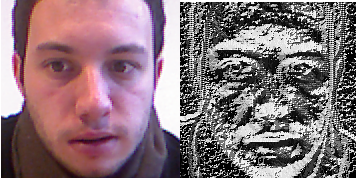
\includegraphics[scale=0.8]{figures/lbp_implementation_example} 
\newline
\caption{Circular LBP operator with $ P = 8 $ and $ R = 1.0 $}
\label{lbp_implementation_example}
\end{center} 
\end{figure}

\noindent The face image is divided into regions. As it is commonly done, the face is a grid pattern of $ 6\times7 $ (6 partitions for the columns and 7 partitions for the rows). In total the face image is divided into 42 regions. For each of these regions, the LBP operator, $ LBP_{8,1}^{u^2} $, computes every pixel.
\newline

\noindent The output of this computation is the number of labelled 1s for the 8 neighbor pixels. Because a uniform LBP operator is used, the number is from 0 to 8. If the number is 9, it means that it is a non-uniform LBP. In total, the output number can have 10 different values (from 0 to 9).
\newline

\phantomsection
\section{Histogram computing}

\vspace{\baselineskip}
\noindent The numbers obtained after computing a region are concatenated into an histogram. The histogram has 10 bins; a bin for each value from 0 to 9. Each bin contains the number of pixels that have the value that correspond to that bin. For example, if in a specific region, 20 pixels, after being computed by the LBP operator are labelled with the value 7, then the bin attributed to the value 7 will have a value of 20 for this specific region. The figure~\ref{lbp_implementation_histogram} shows two pixels with their eight neighbor pixels, a region containing these pixels with the values obtained with the LBP operator and an histogram computed for this region.
\newline

\begin{figure}[!h]
\begin{center}
\noindent 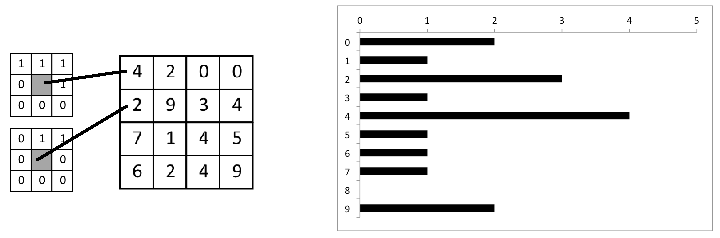
\includegraphics[scale=0.6]{figures/lbp_implementation_histogram} 
\newline
\caption{Example of Histogram computation}
\label{lbp_implementation_histogram}
\end{center} 
\end{figure}

\noindent To obtain the feature vector for the whole image, an histogram is computed for each regions. In total, there are 42 histograms computed for the 42 regions. For the whole image, the 42 histograms have in total 420 bins; 10 bins for each histogram. The feature vector is obtained by putting the histogram side to side. The figure~\ref{lbp_implementation_vector} shows how the feature vector is obtained with all the histograms.
\newline

\begin{figure}[!h]
\begin{center}
\noindent 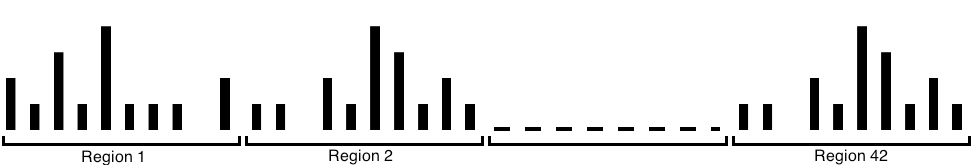
\includegraphics[scale=0.4]{figures/lbp_implementation_vector} 
\newline
\caption{Example of a feature vector composed by the 42 histograms}
\label{lbp_implementation_vector}
\end{center} 
\end{figure}

